Twierdzenie Hall'a jest fajne, ale niestety działa tylko w~grafach dwudzielnych. Przydałby się nam jakiś warunek, który mówi o~istnieniu dopasowania doskonałego w~\emph{dowolnym} grafie.

Powiedzmy, że mamy graf $G$~o $n$~wierzchołkach. Dla uproszczenia będziemy te wierzchołki traktować jako liczby ze zbioru $[n]$, bo wyjdzie na to samo. Dla każdej krawędzi $\{i, j\}$, gdzie $i < j$, zróbmy sobie pewną zmienną, którą będziemy oznaczać $x_{ij}$. Za chwilę wyjaśni się, co to dokładnie znaczy. Następnie zdefiniujemy sobie tzw. \emph{macierz symboliczną Tutte'a}. Jest to macierz $n \times n$, a~wypełniamy ją zgodnie z~poniższą regułą:
\begin{equation*}
	M_G[i, j] = \begin{cases}
		0       & \iff \{i, j\} \not\in E\pars{G}         \\
		x_{ij}  & \iff \{i, j\} \in E\pars{G} \land i < j \\
		-x_{ij} & \iff \{i, j\} \in E\pars{G} \land i > j
	\end{cases}
\end{equation*}

Przykładowo, dla takiego grafu:
\begin{figure}[H]
	\centering
	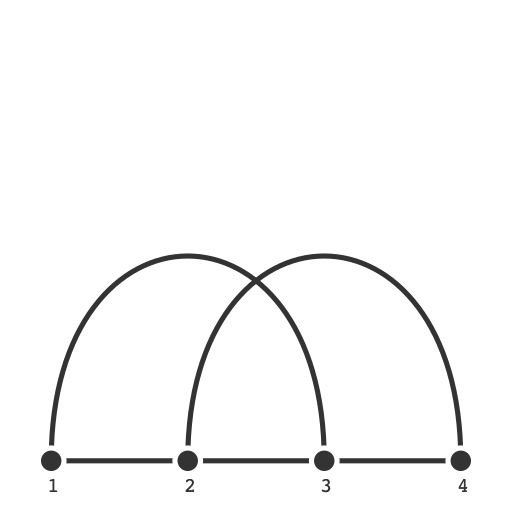
\includegraphics[scale=0.5]{images/tutte/tutte_matrix_example_graph.png}
\end{figure}

będzie
\begin{equation*}
	M_G = \begin{bmatrix}
		0       & x_{12}  & x_{13}  & 0      \\
		-x_{12} & 0       & x_{23}  & x_{24} \\
		-x_{13} & -x_{23} & 0       & x_{34} \\
		0       & -x_{24} & -x_{34} & 0
	\end{bmatrix}
\end{equation*}
Zwróćmy uwagę, że jest to macierz skośnie symetryczna.

Prawdziwe okazuje się:
\begin{theorem}
	Graf $G$~ma dopasowanie doskonałe wtedy i~tylko wtedy, gdy wyznacznik symboliczny macierzy $M_G$ jest niezerowy.
\end{theorem}
Spokojnie, powoli\dots Wyjaśnijmy sobie najpierw, czym jest ten wyznacznik symboliczny. Wyznacznik macierzy będzie (z~definicji) czymś takim:
\begin{equation*}
	\det\pars{M_G} = \sum_{\pi \in S_n}\sgn\pars{\pi} \cdot \pars{\prod_{i = 1}^{n}M_G[i, \pi\pars{i}]}
\end{equation*}
Gdyby w~naszej macierzy $M_G$~były konkretne liczby, to wyznacznik byłby po prostu wartością tego wyrażenia. Ale w~naszej macierzy są bliżej nieokreślone (na razie) zmienne, więc będziemy to wyrażenie traktować jako wielomian tych wszystkich zmiennych $x_{ij}$ odpowiadających krawędziom i~nazwać \emph{wyznacznikiem symbolicznym}. Przez jego ,,niezerowość'' rozumiemy, że ten wielomian nie jest tożsamościowo równy zero. Skoro wyjaśniliśmy już, o~czym mówi to (na pierwszy rzut oka losowe) twierdzenie, to możemy przystąpić do jego dowodzenia.
\begin{proof}
	Najpierw zaobserwujmy, o~czym mówi nam wyznacznik symboliczny. Iterujemy się tam po wszystkich permutacjach $\pi \in S_n$. Wiadomo, że każda permutacja rozkłada się na rozłączne cykle. Okazuje się, że każda permutacja, dla której wyrażenie pod sumą się nie zeruje, odpowiada pewnemu skierowanemu pokryciu cyklowemu $G$. Co to jest pokrycie cyklowe? Najprościej mówiąc: bierzemy sobie kilka rozłącznych wierzchołkowo cykli w~$G$ w~taki sposób, żeby każdy wierzchołek $G$ należał do jakiegoś wybranego cyklu. Ponieważ mówimy o~\emph{skierowanym} pokryciu cyklowym, to jedna krawędź nieskierowana może się liczyć jako cykl długości $2$, z~krawędziami skierowanymi w~obydwie strony. Poniżej przykładowy graf i~pewne jego pokrycie cyklowe:

	\begin{figure}[H]
		\centering
		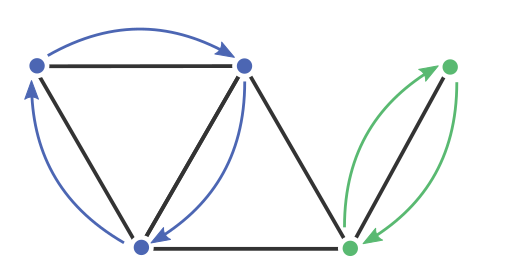
\includegraphics[scale=0.75]{images/tutte/decomposed_graph.png}
		\caption{Przykładowe pokrycie cyklowe}
	\end{figure}

	Mając tę intuicję, faktycznie widzimy, że permutacja $\pi$, dla której wyrażenie pod sumą się nie zeruje, odpowiada pokryciu cyklowemu. Gdyby bowiem nie było to pokrycie cyklowe, to nie istniałaby w~$G$ któraś krawędź postaci $\pars{i, \pi\pars{i}}$. Ale wtedy, z~definicji $M_G$, byłoby $M_G[i, \pi\pars{i}] = 0$, czyli jednak składnik odpowiadający $\pi$ zerowałby się. Zatem tak naprawdę:
	\begin{equation*}
		\det\pars{M_G}
		= \sum_{\pi \in S_n}\sgn\pars{\pi} \cdot \pars{\prod_{i = 1}^{n}M_G[i, \pi\pars{i}]}
		= \sum_{\substack{\pi \in S_n\\\text{\tiny $\pi$ --- pokr. cykl. $G$}}}\sgn\pars{\pi} \cdot \pars{\prod_{i = 1}^{n}M_G[i, \pi\pars{i}]}
	\end{equation*}

	Z~tego od razu możemy wyprowadzić dowód w~jedną stronę. Załóżmy, że istnieje skojarzenie doskonałe w~$G$ i, bez straty ogólności, składa się ono z~krawędzi $\{1, 2\}, \{3, 4\}, \ldots, \{2k - 1, 2k\}$, gdzie $2k = n$. Skoro to skojarzenie doskonałe, to te krawędzie nie dotykają się wierzchołkami, zatem możemy zrobić pokrycie wierzchołkowe transpozycjami $\pars{1, 2}, \pars{3, 4}, \ldots, \pars{2k - 1, 2k}$, jak na poniższym rysunku:

	\begin{figure}[H]
		\centering
		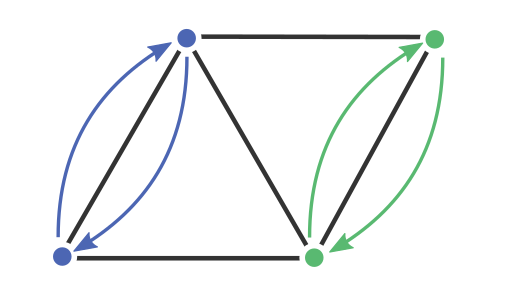
\includegraphics[scale=0.75]{images/tutte/perfect_matching_cover.png}
		\caption{Pokrycie cyklowe zrealizowane za pomocą transpozycji}
	\end{figure}

	W~wyznaczniku symbolicznym składnik odpowiadający permutacji opisującej to pokrycie cyklowe będzie wyglądał następująco:

	\begin{equation*}
		x_{12} \cdot \pars{-x_{12}} \cdot x_{34} \cdot \pars{-x_{34}} \cdot \ldots \cdot x_{2k - 1\ 2k} \cdot \pars{-x_{2k - 1\ 2k}}
	\end{equation*}

	i~po prostu widać, że nic się z~tym nie zredukuje, bo są tu tylko transpozycje, więc jeśli nawet je odwrócimy to nic się nie zmieni --- w~szczególności znak tego wyrażenia. Zatem faktycznie wyznacznik symboliczny nie będzie tożsamościowo równy zero.

	Dowód w~drugą stronę, tzn.: jeśli wyznacznik symboliczny nie jest tożsamościowo równy zero, to mamy skojarzenie  doskonałe, jest nieco bardziej skomplikowany, ale opiera się na naturalnej obserwacji:
	\begin{equation*}
		\begin{split}
			\det\pars{M_G}
			&= \sum_{\pi \in S_n}\sgn\pars{\pi} \cdot \pars{\prod_{i = 1}^{n}M_G[i, \pi\pars{i}]}
			= \sum_{\substack{\pi \in S_n\\\text{\tiny $\pi$ --- pokr. cykl. $G$}}}\sgn\pars{\pi} \cdot \pars{\prod_{i = 1}^{n}M_G[i, \pi\pars{i}]}\\
			&= \pars{\sum_{\substack{\pi \in S_n\\\text{\tiny $\pi$ -- pokr. cykl. $G$}\\\text{\tiny $\pi$ bez niep. cykli}}}\sgn\pars{\pi}\pars{\prod_{i = 1}^{n}M_G[i, \pi\pars{i}]}} + \pars{\sum_{\substack{\pi \in S_n\\\text{\tiny $\pi$ -- pokr. cykl. $G$}\\\text{\tiny $\pi$ ma niep. cykle}}}\sgn\pars{\pi}\pars{\prod_{i = 1}^{n}M_G[i, \pi\pars{i}]}}
		\end{split}
	\end{equation*}
	Jak nam to pomaga? Zauważmy, że druga suma się zeruje. Dlaczego? Otóż dla każdej permutacji, w~której istnieje nieparzysty cykl, możemy wziąć nieparzysty cykl zawierający najmniejszą liczbą i~go odwrócić. Np. z~poniższej permutacji $\pi$:

	\begin{figure}[H]
		\centering
		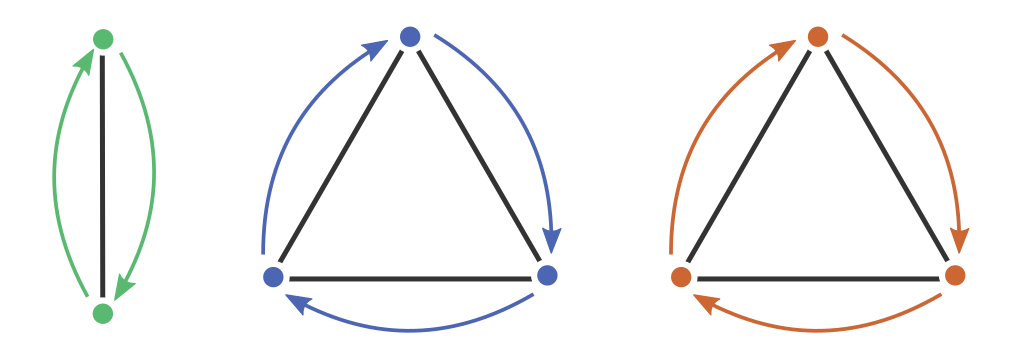
\includegraphics[scale=0.5]{images/tutte/pre_switching.png}
		\caption{Permutacja $\pi = (1, 2)(3, 4, 5)(6, 7, 8)$}
	\end{figure}

	powstanie permutacja $\pi'$:

	\begin{figure}[H]
		\centering
		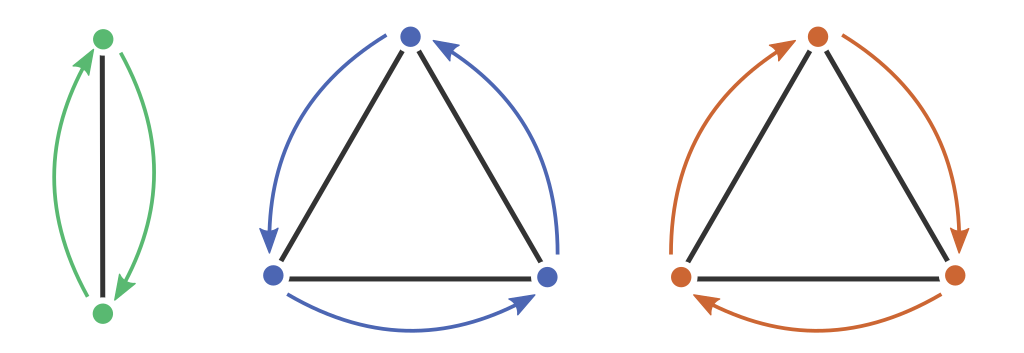
\includegraphics[scale=0.5]{images/tutte/post_switching.png}
		\caption{Permutacja $\pi' = (1, 2)(5, 4, 3)(6, 7, 8)$}
	\end{figure}

	To przekształcenie jest oczywiście bijekcją (i~dodatkowo inwolucją). Zauważmy też, że składnik sumy odpowiadający $\pi'$ różni się tylko znakiem od składnika sumy odpowiadającego $\pi$ --- końce krawędzi przecież się nie zmieniły, jedynie dla każdej zmiennej odpowiadającej krawędzi zmienił się znak, bo krawędź zmieniła kierunek. A~cykl był nieparzystej długości, co oznacza, że zmieniło się nieparzyście wiele znaków. Zatem składnik dla $\pi$ zredukuje się ze składnikiem dla $\pi'$ dla dowolnej permutacji $\pi$, w~której istnieje nieparzysty cykl, czyli rzeczywiście cała druga suma się wyzeruje. Ale założyliśmy, że wyznacznik symboliczny jest niezerowy, czyli pierwsza suma jest niezerowa. Oznacza to, że istnieje pokrycie cyklowe $G$, w~którym nie ma nieparzystych cykli --- innymi słowy, są same parzyste. Zauważmy teraz, że ponieważ są to rozłączne cykle parzystej długości pokrywające $G$, to, biorąc co drugą krawędź z~każdego takiego cyklu, otrzymamy dopasowanie doskonałe:

	\begin{figure}[H]
		\centering
		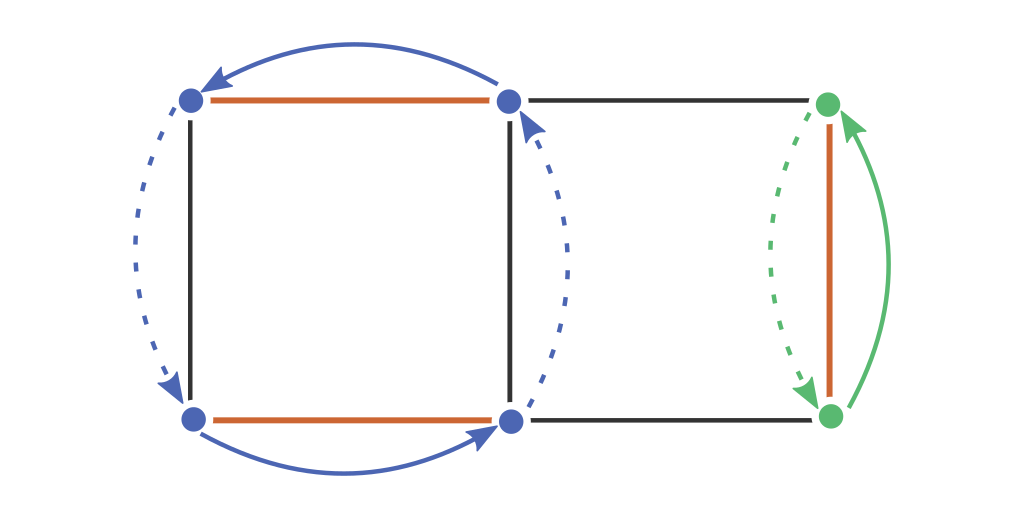
\includegraphics[scale=0.75]{images/tutte/matching_from_cover.png}
		\caption{Pokrycie cyklowe oraz skojarzenie doskonałe; linia ciągła oznacza krawędź cyklu, którą bierzemy do skojarzenia }
	\end{figure}

	A~to właśnie chcieliśmy pokazać!
\end{proof}